%exploring
\documentclass[hidelinks,12pt,a4paper]{report}
\usepackage[toc,page]{appendix}

%%Links
\usepackage{hyperref}

%%Including code
\usepackage{holtex}
\usepackage{holtexbasic}
\usepackage{enumerate}
\usepackage{listings}
\usepackage{pdfpages}

%% Acronyms
\usepackage[acronym,toc]{glossaries}
\loadglsentries{acronyms}
\makenoidxglossaries
\usepackage[nolist,nohyperlinks,printonlyused,nonumberlist]{acronym}

%%Section numbering
\usepackage{subfiles}
\usepackage{blindtext}
\setcounter{secnumdepth}{4}
\setcounter{tocdepth}{4}

%% References
\usepackage[nottoc]{tocbibind}
\renewcommand{\bibname}{References}

%% Graphics
\usepackage{graphicx}
\graphicspath{{../figures/}}

%%%%%%%% Style
\renewcommand{\contentsname}{Table Of Contents}
\pagenumbering{roman}
\usepackage{geometry}
\geometry{
right=1in,     rmargin=1in,
left=1in,       lmargin=1in,
top=1in,       tmargin=1in,
bottom=1in, bmargin=1in,
marginparwidth=0in
}
\usepackage{setspace}

\usepackage{textgreek}


%%%%%%%%%%%%%% Document %%%%%%%%%%%%%%%%%%%%%
\begin{document}
\lstset{language=ML, basicstyle=\scriptsize}
\title{Certified Security by Design (CSBD) Applied to United States Army Ranger Patrol Base Operations: An Example of Formal Verification of Complete Mediation Applied to A Non-automated, Human-Centered System}
\author{Lori Pickering}

%\frontmatter
%% Testing figure placement and inclusion in List of Figures
\begin{figure}[t]
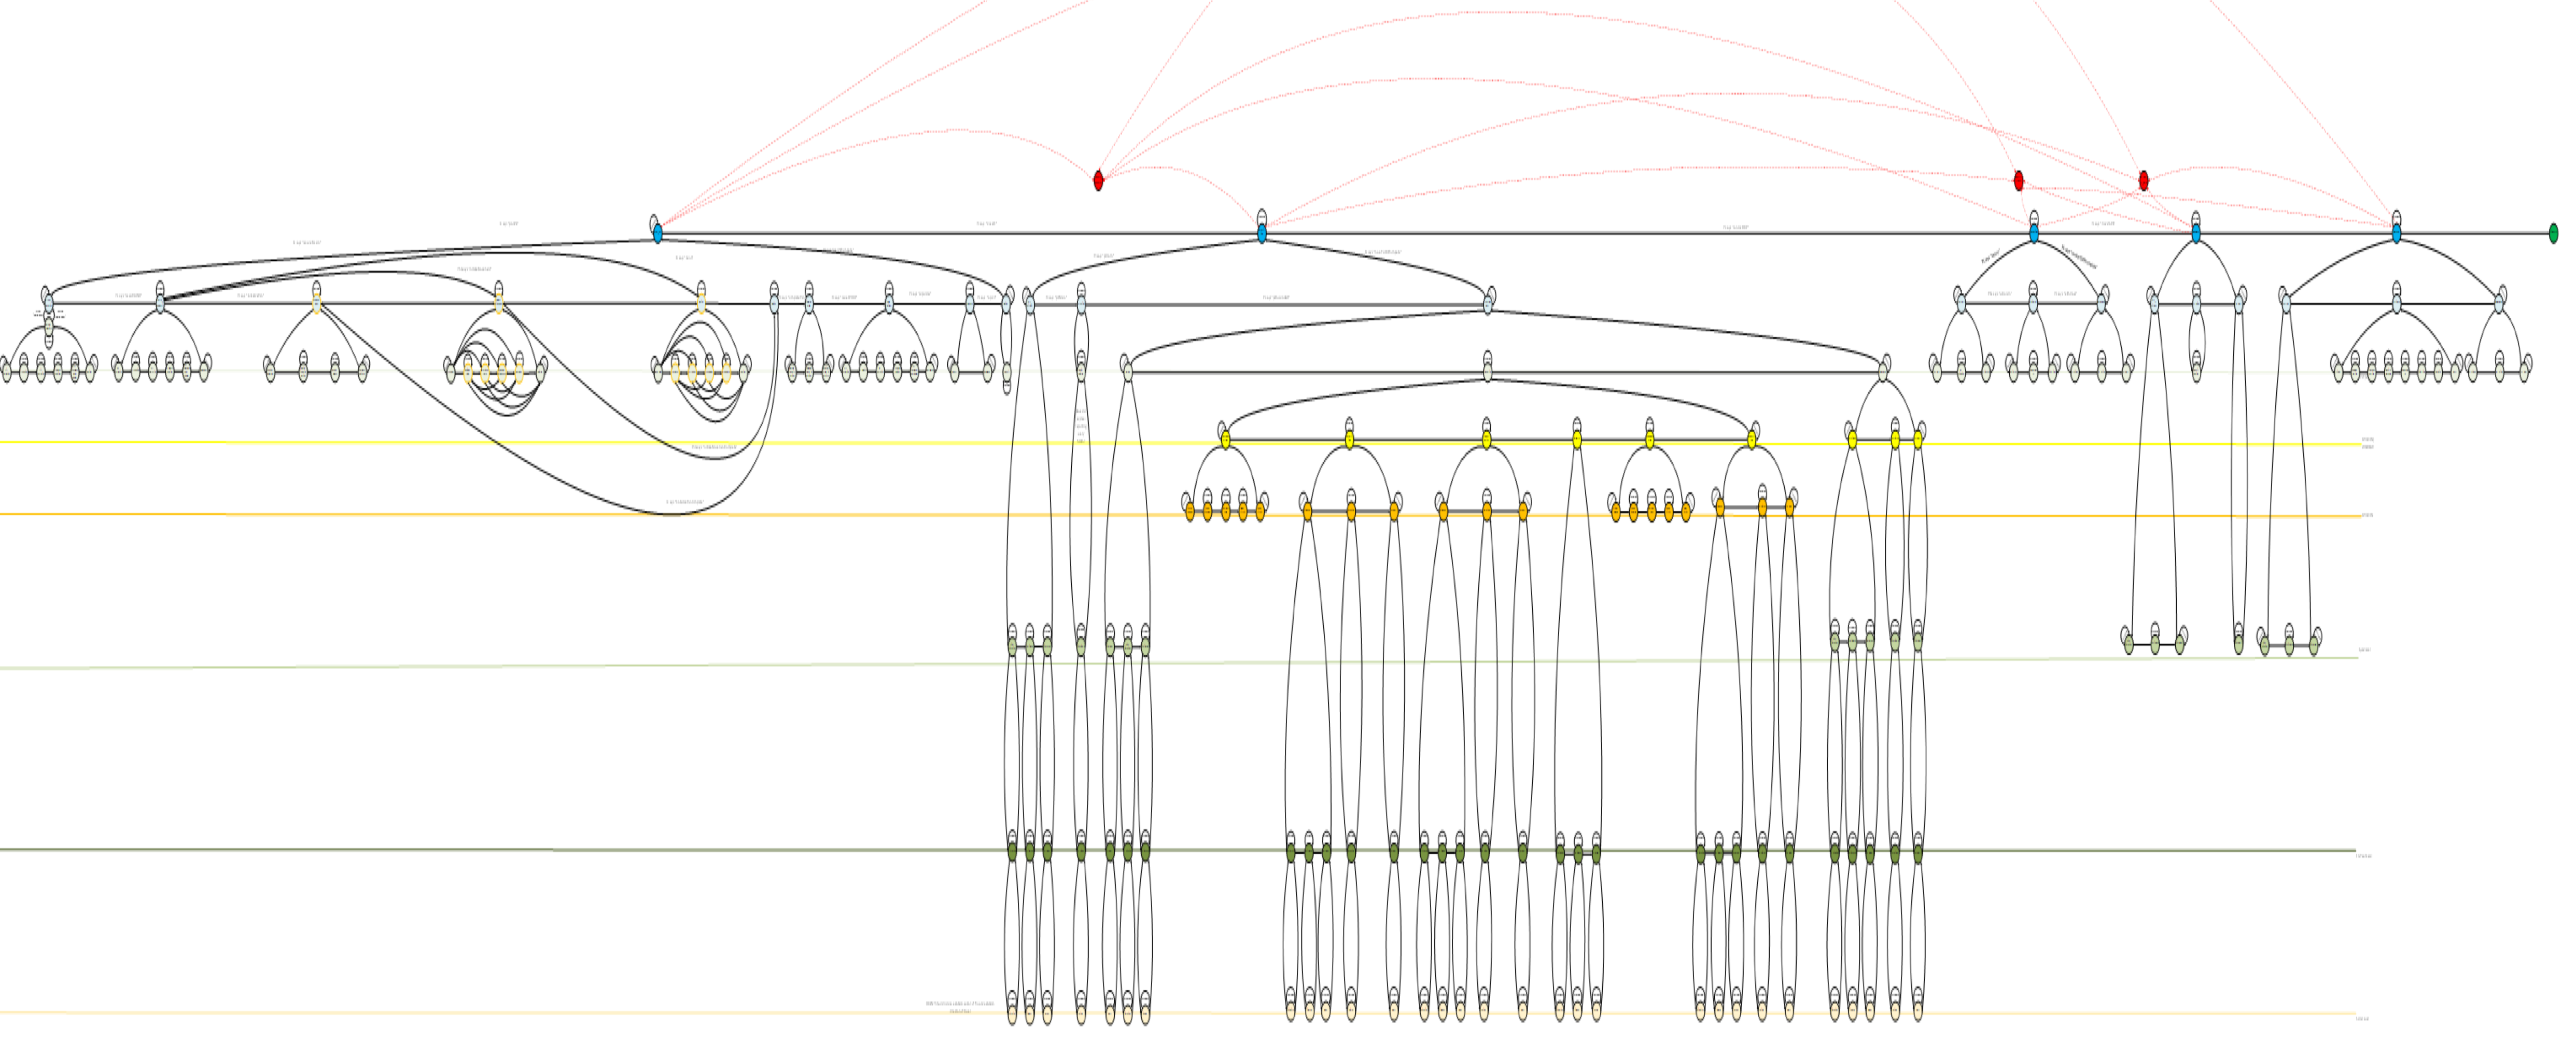
\includegraphics[width=\textwidth]{../figures/overalldiagramsquashed.png}
\caption{This is a caption for this figure.}
\end{figure}

\begin{doublespace}
\cleardoublepage \phantomsection
\addcontentsline{toc}{chapter}{Abstract}
\subfile{../frontMatter/abstract/abstract}
\setcounter{page}{1}
\end{doublespace}
\cleardoublepage \phantomsection
\subfile{../frontMatter/frontMatter}
%%%%%%%%% TOC %%%%%%%%%%%%%%%%%%%%%%%%%%%%
\tableofcontents
\cleardoublepage



\hypersetup{
  colorlinks   = true, %Colours links instead of ugly boxes
  urlcolor     = blue, %Colour for external hyperlinks
  linkcolor    = blue, %Colour of internal links
  citecolor   = red %Colour of citations
}

%%%%%%%%% Figures, Tables, Acronyms %%%%%%%%%%%%%%%%%
\cleardoublepage \phantomsection
\listoffigures

\cleardoublepage \phantomsection
\listoftables

\cleardoublepage
%\addcontentsline{toc}{chapter}{List of Acronyms}
%\subfile{../frontMatter/listOfAcronyms/listOfAcronyms}
\printnoidxglossary[type=\acronymtype, title={List of Acronyms}]
\cleardoublepage

%%%%%%%%% Main Matter %%%%%%%%%%%%%%%%%%%%%%%
\parskip=18pt
\raggedright

\begin{doublespace}
\subfile{../chapters/introduction/introduction}
\pagenumbering{arabic}
\cleardoublepage

\subfile{../chapters/background/background}
\cleardoublepage

\subfile{../chapters/sse/sse}
\cleardoublepage

\subfile{../chapters/csbdacl/csbdacl}
\cleardoublepage

\subfile{../chapters/pb/pb}
\cleardoublepage

\subfile{../chapters/ssms/ssms}
\cleardoublepage

\subfile{../chapters/pbssm/pbssm}
\cleardoublepage

\subfile{../chapters/discussion/discussion}
\cleardoublepage

\subfile{../chapters/future/future}
\cleardoublepage
\end{doublespace}
\cleardoublepage


%%%%%%% Appendicies %%%%%%%%%%%%%%%%
\begin{appendices}
\chapter{Access Control Logic Theories: Pretty-Printed Theories}
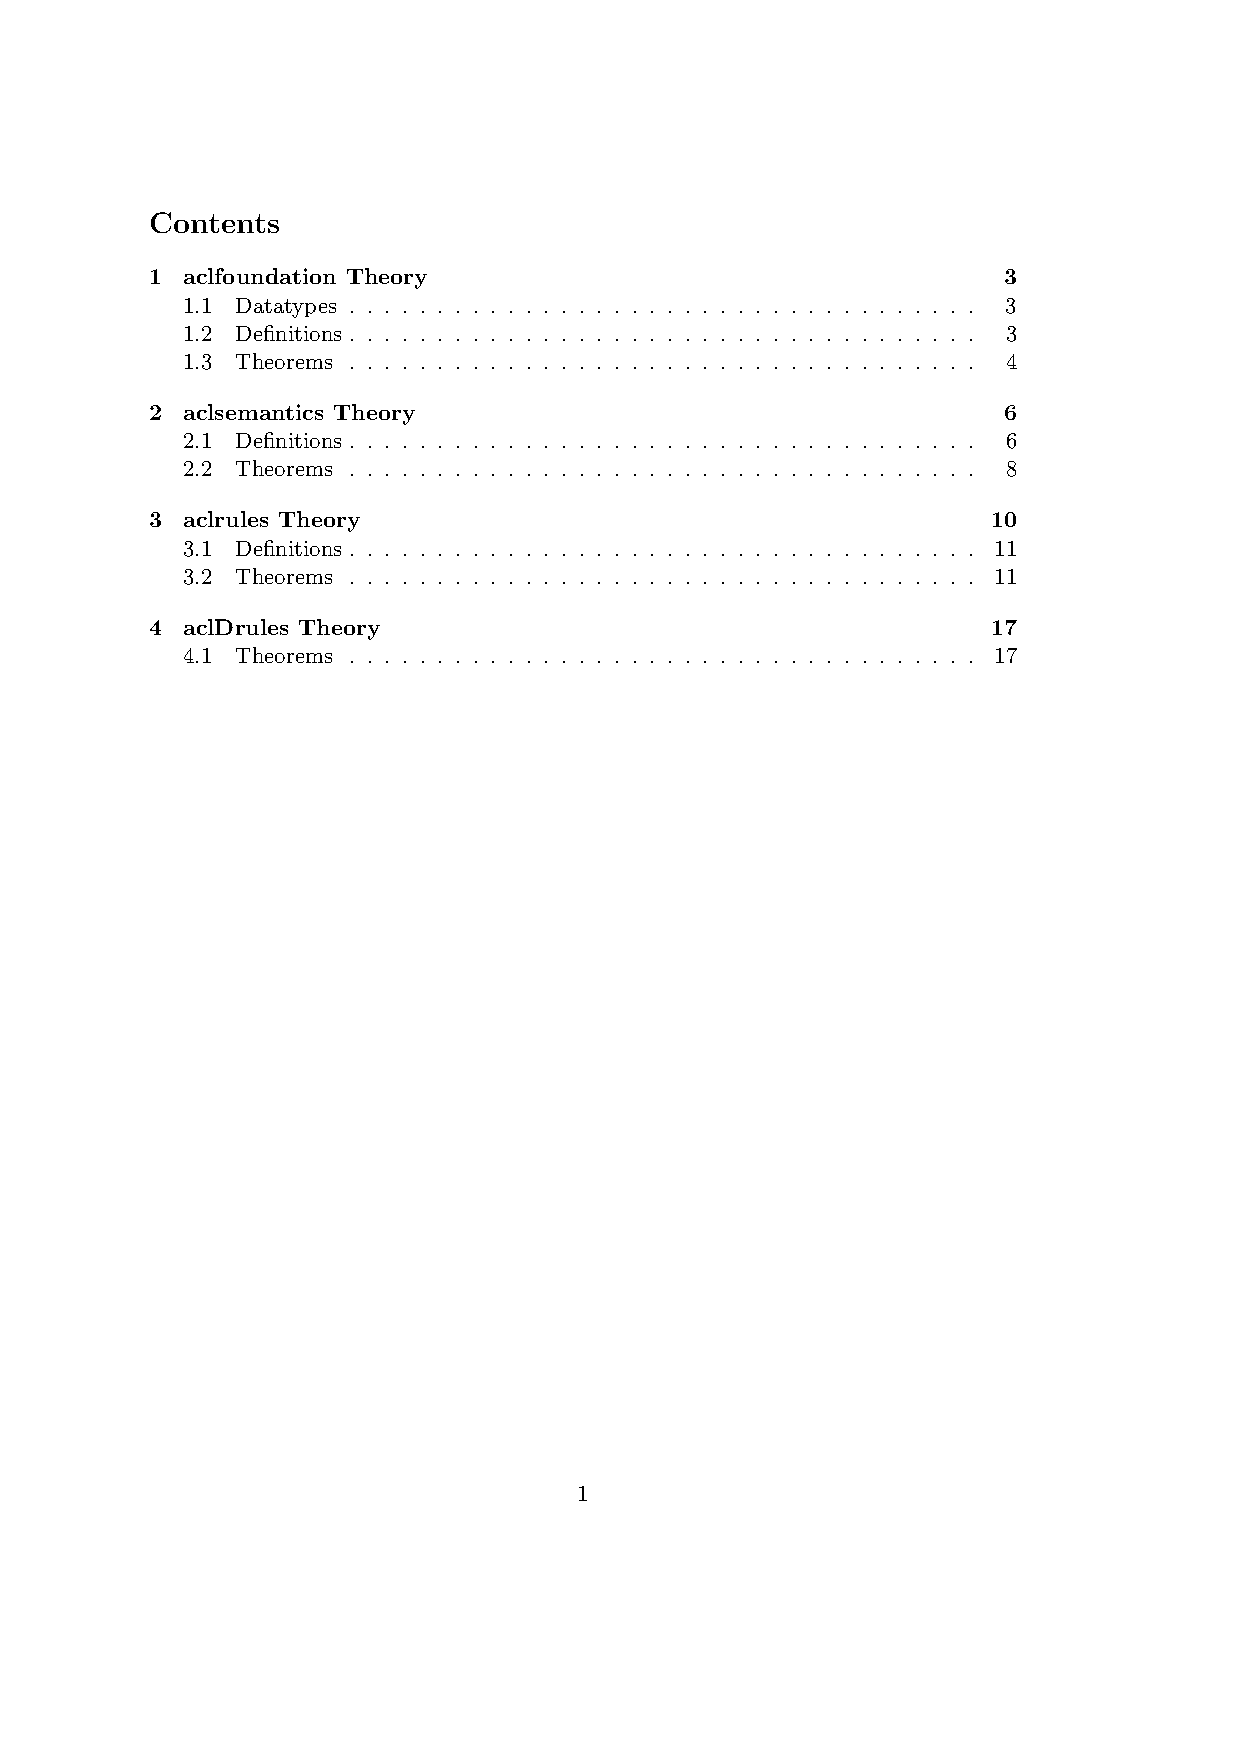
\includepdf[pages=-]{../../HOL/ACL/HOLReports/aclReport.pdf}

\chapter{Secure State Machine \& Patrol Base Operations: Pretty-Printed Theories }
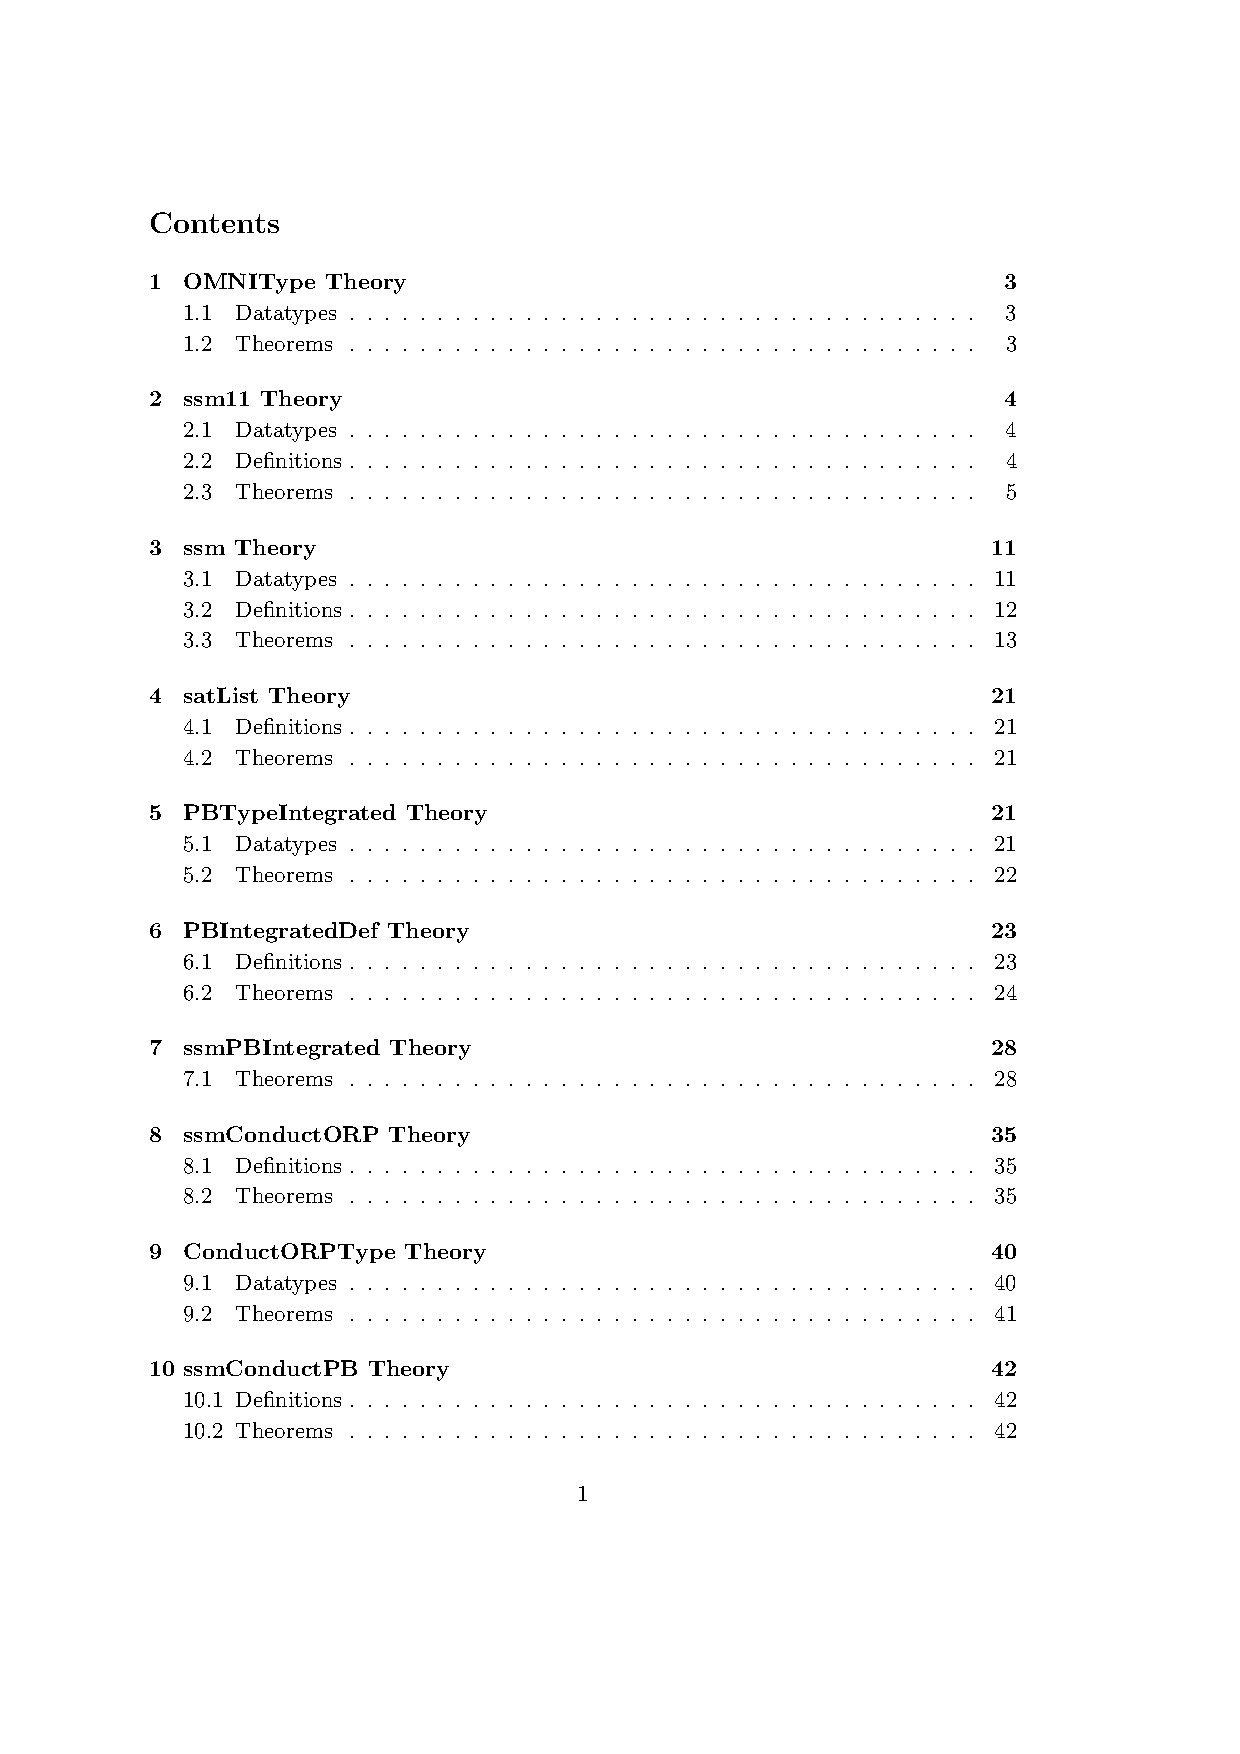
\includepdf[pages=-]{../../HOL/HOLReportsOMNI/OMNIReport.pdf}

\chapter{Secure State Machine Theories: HOL Script Files}
\section{ssm}
\lstinputlisting{../../HOL/ssms/ssmScript.sml}
\section{satList}
\lstinputlisting{../../HOL/ssms/satListScript.sml}


\chapter{Secure State Machine Theories Applied to Patrol Base Operations: HOL Script Files}
\section{OMNILevel}
\lstinputlisting{../../HOL/OMNILevel/OMNIScript.sml}

\section{TopLevel}
\subsection{PBTypeIntegrated Theory: Type Definitions}
\lstinputlisting{../../HOL/topLevel/PBTypeIntegratedScript.sml}
\subsection{PBIntegratedDef Theory: Authentication \& Authorization Definitions}
\lstinputlisting{../../HOL/topLevel/PBIntegratedDefScript.sml}
\subsection{ssmPlanPBIntegrated Theory: Theorems}
\lstinputlisting{../../HOL/topLevel/ssmPBIntegratedScript.sml}


\section{Horizontal Slice}
\subsection{ssmPlanPB}
\subsubsection{PlanPBType Theory: Type Definitions}
\subsubsection{PlanPBDef Theory: Authentication \& Authorization Definitions}
\subsubsection{ssmPlanPB Theory: Theorems}

\subsection{ssmMoveToORP}
\subsubsection{MoveToORPType Theory: Type Definitions}
\subsubsection{MoveToORPDef Theory: Authentication \& Authorization Definitions}
\subsubsection{ssmMoveToORP Theory: Theorems}

\subsection{ssmConductORP}
\subsubsection{ConductORPType Theory: Type Definitions}
\subsubsection{ConductORPDef Theory: Authentication \& Authorization Definitions}
\subsubsection{ssmConductORP Theory: Theorems}

\subsection{ssmMoveToPB}
\subsubsection{MoveToPBType Theory: Type Definitions}
\subsubsection{MoveToPBDef Theory: Authentication \& Authorization Definitions}
\subsubsection{ssmMoveToPB Theory: Theorems}

\subsection{ssmConductPB}
\subsubsection{ConductPBType Theory: Type Definitions}
\subsubsection{ConductPBDef Theory: Authentication \& Authorization Definitions}
\subsubsection{ssmConductPB Theory: Theorems}


\section{Vertical Slice}
\subsection{ssmSecureHalt}
\subsubsection{SecureHaltType Theory: Type Definitions}
\subsubsection{SecureHaltDef Theory: Authentication \& Authorization Definitions}
\subsubsection{ssmSecureHalt Theory: Theorems}

\subsection{ssmORPRecon}
\subsubsection{ORPReconType Theory: Type Definitions}
\subsubsection{ORPReconDef Theory: Authentication \& Authorization Definitions}
\subsubsection{ssmORPRecon Theory: Theorems}

\subsection{ssmMoveToORP4L}
\subsubsection{MoveToORP4LType Theory: Type Definitions}
\subsubsection{MoveToORP4LDef Theory: Authentication \& Authorization Definitions}
\subsubsection{ssmMoveToORP4L Theory: Theorems}

\subsection{ssmFormRT}
\subsubsection{FormRTType Theory: Type Definitions}
\subsubsection{FormRTDef Theory: Authentication \& Authorization Definitions}
\subsubsection{ssmFormRT Theory: Theorems}

\chapter{Map of The File Folder Structure}

\end{appendices}\cleardoublepage

%%%%%%%%%% References %%%%%%%%%%%%%%%%%%%%%
\bibliographystyle{unsrt}
\bibliography{mtref}
\doublespacing
\end{document}